\section{インベスターKへの手紙}
\rightline{（文責:京都大学難平同好会）}

\subsection{はじめに}
　「お金あるある：ない」　というジョークが世に出て久しいが、こと熊野寮生に関してはあるあるどころかもはや不変の原理である。京都大学はそのような学生に学びの機会を恵んできたはずであるが、昨今の廃寮化攻撃や授業料免除廃止等を見るにこれからも生かしてもらえると考えるのは些か楽観的過ぎるというものだ。昨今の政府は「自助」を我々に課しており、その最たるものはＮＩＳＡというやつである。金のない人間に金を供託させるなど福利厚生として成立しているか怪しいものであるが、とにかくまあ用意されているならこれを活用しない手はない。この文章は私が大学生活6年間を通して行った投資の振り返りである。投資する金がある程度の貧者は参考にしてほしい。金が余って仕方ない人間はこんなもの読まずに宝くじでも買っていればよい。

\subsection{おことわり}
　この文章は投資を推奨するものではない。また、この文章を読んであなたがどのような損害を被っても責任は負わないし、記載された銘柄の変動によって筆者が利益を得る可能性も否定しない。自己判断で投資を行うこと。
　また、勘違いをしてもらっては困るのだがそもそも私は投資と投資家が嫌いである。通帳の残高は人生ゲームのスコアではなく、顔も知らない子供の人生を潰して絞った汁だと胸に刻んでおくように。
　さらには学生時代の株式投資は（得られる経験に関する評価を無視すれば）あまりにも非効率であることも理解しなくてはならない。投資では時間を味方につけて～などと言われるが入金し続けられる前提である。学生時代の貴重な資金が４年ロックされて３割ほど増えたとてなんの意味があるかよく考えてから投資せよ。

\subsection{方針}
開始時点での投資方針はおおよそ以下のものである
１．イオン（８２６７）の購入をひとまずのゴールとする
２．投資信託のカード積み立てを継続する

　１に関してだが、当時は１００株で２０万円ほどであった本銘柄は、株主優待で半年ごとに最大３万円のキャッシュバックを現金で受け取ることができた。これは配当と値上がりを考慮せずに年利３０％に相当する圧倒的なリターンを誇るうえになんと非課税である（厳密には違うが）。いわゆる”エッジ”であったものの現在は３倍近く値上がりし１００株７０万円を超えており”塞がれる”ことになった。

　また、２に関してだが、私が利用している楽天証券にはカードで積み立てると投資額の０．５％が楽天ポイントとして帰ってくるというサービスがある。ところでこのポイントは投資信託の購入に充てることができるため売買手数料の発生しない商品を介せば完全に日本円と等価になる。銀行の利息が年利０．０５％の時代に月０．５％でいきなり利益が生じる。投信の積み立てと合わせて同額解約すると価格変動リスクを踏み倒すことができるが、めんどくさいので実行しなかった。少し生活が苦しくなる程度の額を積み立てて必要な時は売却するスタイルがちょうどいいか。毎月寮食が１日無料になる程度の恩恵がある。

　以上２点はいずれも世間一般に知られる投資手法よりも格段に強力であるが、代わりに入金額によって利益を伸ばしづらいという点がある。イオンは１００株からこのリターンを得られるがキャッシュバックを１万円増やそうとすると５倍の株を保有する必要があるし投信積立は月１０万円の上限がある。少額投資の方が有利になる投資法をかき集めれば我々でも一段飛ばしで資産を積み上げられるはずだ。

\subsection{運用履歴}
\subsubsection{米国株分散投資時代（２０２１～）}
　当時はまだ投資ブームなるものが来ていなかったため幾分か有用な情報がネット上でも得られた。情報をもとに私が組んだポートフォリオが以下のものである。

\begin{figure}[h]
  \centering
  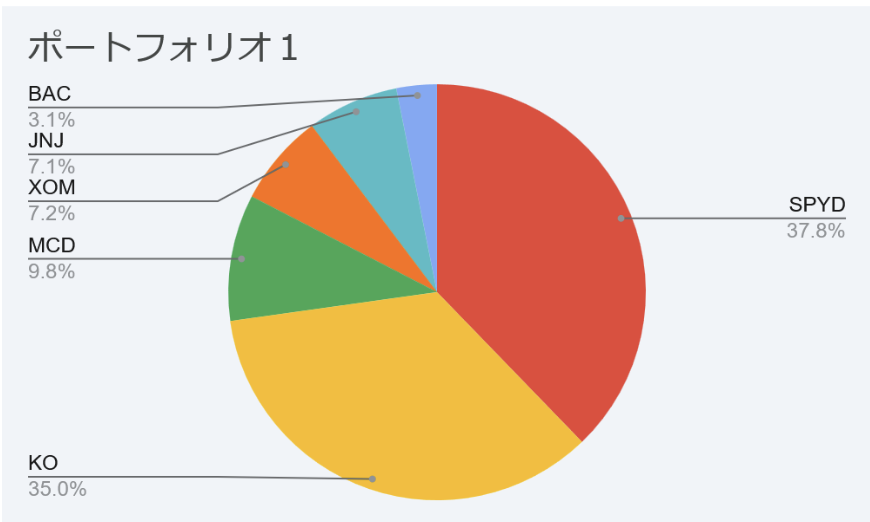
\includegraphics[width=0.8\linewidth]{2026shinki/invester_k/portfolio1.png}
  \caption{最初のポートフォリオ}
\end{figure}

　SPYDをコアとしてKO、MCD、JNJなど王道の銘柄が並ぶ。「米国株は日本株より優れている」のスローガンのもとに全額を米株に投資していた時代である。なお、グラフには含まれていないが実際にはSP500投資信託に積み立ても行っていることにも留意されたい。この時点での総資産は２０万円ほどで入学までの貯金や入学祝、コロナ情勢による学生給付金（いわゆるアベの１０万）を財源とした。
また、この時期はいわゆるコロナショックからの回復期にあり急激な株高にあったため幸か不幸か株初心者にしていきなり黄金時代を経験することになる。多少のリバランスを行いながらセクター別ETFへと移行し、安定した運用を行うことができた。

\subsubsection{短期トレード時代（～２０２２.３月）}
　実家からの仕送りやアルバイトの給料、あるいは配当金がたまって来るころ、私は新たな戦術に活路を見出した。ロシアによる侵攻、依然として残るコロナへの恐怖といった要因で日々大きな変動を見せる銘柄―原油と半導体の短期取引である。買って―上がったら―売る。極めて初歩的な取引だが実際これはかなりの利益をもたらした。単元株が安い（当時一株450円程）という理由だけでENEOSを好んで運用したが、この銘柄一本でキャピタル１０万円、インカム２万円は稼げたため判断は（偶然ではあるが）正しかったといえる。
　ところで、短期取引を行うにあたって一般投資家には制限がある。「一つの銘柄は一日に一往復しかできない」というものだ。一度購入して売却するとその取引で得られた資金は同じ銘柄の購入には充てることができず、再び買うためにはまだ手を付けていない残高が残っている必要がある。この制限がないと差金取引になるためだ。このせいで通常一日に稼げる額が頭打ちになるのだが、回避策として私が考案したのがはしご取引である。あらかじめ複数の短期取引用銘柄をリストアップしておき順番に買売（はしご）することで制限にとらわれず取引ができる。私はENEOS->INPEX->日鉄->HCキャピタルのリストを気に入っていた。これらの銘柄は低PBRであるために最悪底値掴みしてもそのうち上昇するという精神安定剤の側面も備えていた。取引は好調で月末には資産が９０万円に達しようとしていた。

\subsubsection{幕開け（２０２２・４/５～）}
　順調に保有資産が指数関数のグラフを描き一般学生に似つかわしくない取引を繰り返すようになった私は新たな値上がり銘柄を求めて情報収集に励んでいた。おそらく何らかの投資ブログだったであろうか、素晴らしい成長性と安定性を秘めた銘柄があるというではないか！！！私は有り金をすべてはたいて当該銘柄を買いあさったのである。毎日何万という含み益が生まれ、不労所得の甘美に酔いしれる生活を送ることとなる―なんて素晴らしい！。


　～時は流れ４月２６日～
　株に明るくない私はこの日決算が発表されることも知らずのんきに大学なんぞに行っていたのである。夕方になり飯を食い終え日課の株価チェックで端末を見ると資産が半分ほどになっている。間違えて売ったかと銘柄のページを見に行くと板にはSの文字が―ストップ安である。そこで初めて私の資産はイナゴに食いつくされたのだと気づく。結局翌日に成行で売り注文をかけ３０万円程の損失で撤退した。無事に売れた喜びと３０万円という額の大きさから来る恐怖の入り混じった得体のしれぬ気分故私は１日布団から出られなかった。しかし、初心者投資家から暴落を経験した中級投資家への幕が開けたという意味も込めて本暴落をマクアケショックと呼称し、糧とすることにした。
　
　とはいえ、手元にはまだ６０万程のキャッシュがあり、まだ復活は可能である。まずは当初の目標であったイオンを購入し、はしご取引で資産を取り戻していった。また、投資で勝つためのルールを定めることにした。

１．イオンは絶対に売らない
２．一つの銘柄が占める割合が３割を超えてはならない
３．東証プライム銘柄のみ購入する

ルール自体はばかげているがこれを機に再びポートフォリオ構築を意識するようになった。コア資産としてイオンを固定し、成長枠としてトヨタなど、その他枠で短期取引という戦術にたどり着く。インカムとキャピタルの両取りを狙ってJリートも仕込むようになった。

　余談ではあるがこの銘柄は現在さらに半額ほどにまで落ちており、損切りしなければ震えるどころではすまなかっただろう。

\subsubsection{投資疲れ、積み立てへ（２０２３～）}
　一日中株価のことを考えて生活していると流スタに疲弊も無視できなくなってくる。授業も手につかず成績は右肩下がりで卒業も逃してしまった。そんな状態なので伝統的な戦術、気絶投資法に手を出すことにした。毎月SP５００とBNDを積み立てて、手を付けない、株価も見ない。退屈だが最強の投資術と呼ばれるだけあり順当に資産が増えていった。
　途中で任天堂などの一部銘柄を保有するなどして遊んだ結果年末にはマクアケショックの負け分を取り返し資産は１５０万円に迫るほどだった。

\subsubsection{歴史は繰り返す（２０２４～）}
　順当に資産を増やしてきた私はさらなる利益を求めて経済に関して情報を収集し始めた。当時はアメリカのインフレが緩やかになりつつあるといった情勢で度重なる利上げの末債券価格は暴落していた。安定資産たる債権がここまで下がっているならもはや買い時ではないかと考えた私は早速資金を調達し三倍債権ETF（TMF）を大量購入、さらにはリセッション対策としてPFEをポートフォリオに加える。利下げが来れば人生逆転できると信じるTwitter上のTMF界隈を心の支えとして粘るも３倍ETF特有の減衰に耐えられずTMF、PFEを全額売却。合計１４０万円ほどで２０万円の赤字を出すことになった。
　利下げ一点読みのTMFはポートフォリオの大部分を占める程信用できる商品ではなく素直にSPXLでも買っていたほうが幾分かましだっただろう。また、ヘルスケアが不況に強いからPFEを買ったが製薬会社をヘルスケアのくくりでとらえてディフェンシブ銘柄とみなすのは論外である。当該は特許切れによるリスクによって株価が低迷していた。高い配当金に目がくらんだためにいらぬ損失を出してしまった点も反省しなくてはならない。

\subsection{結論（２０２５～）}
　人間が株に触れれば必ず欲が出る、感情で取引する。人間は株に向いていない。積み立て以外による注文を原則禁止として至高のポートフォリオを構成した。

～イオン、松屋を優待目的で常に握りNTT、BND、オルカンを毎月積み立てる。資金に余裕が出れば関西電力とサイバーエージェントを交互に購入する～

これが私の考える結論ポートフォリオである。実際のところ松屋は天井で掴んだため塩漬けしているだけだが。


\subsection{おわりに}

　このように紆余曲折を経て私は結局「凡人はインデックス投資をやれ」などというオマハの老人とほぼ同様の結論に至ってしまったわけである。とはいえ得られた経験と多少の収入を加味すればこの６年はSP500をアウトパフォームしたと評価できるだろう。

参考：投資6年の成果
国内株：実現：-150,000　評価：630,000
米国株：実現：-130,000　評価： 10,000
投資信託：実現：30,000 評価：40,000
配当：150,000
その他（イオン優待等）：150,000

計：＋730,000円